\documentclass[10pt,preprint]{sigplanconf}

\usepackage{ifthen}
\usepackage{fancyvrb}
\usepackage{color}
\usepackage{wrapfig}
\usepackage{ulem}
\usepackage{xspace}
\usepackage{relsize}
\usepackage{epsfig}
\usepackage{amssymb}
\usepackage{amsmath}
\usepackage{amsfonts}
\usepackage[utf8]{inputenc}
\usepackage{setspace}
\usepackage[colorinlistoftodos]{todonotes}

\usepackage{listings}

\usepackage[T1]{fontenc}
\usepackage[scaled=0.81]{beramono}


\definecolor{commentgray}{rgb}{0.3,0.3,0.3}

\lstset{
  basicstyle=\ttfamily\footnotesize,
  language=Python,
  keywordstyle=\bfseries,
  stringstyle=\color{blue},
  commentstyle=\color{commentgray}\textit,
  fancyvrb=true,
  showstringspaces=false,
  %keywords={def,while,if,elif,return,class,get,set,new,guard_class}
  numberstyle = \tiny,
  numbersep = -20pt,
}

\newboolean{showcomments}
\setboolean{showcomments}{true}
\ifthenelse{\boolean{showcomments}}
  {\newcommand{\nb}[2]{
    \fbox{\bfseries\sffamily\scriptsize#1}
    {\sf\small$\blacktriangleright$\textit{#2}$\blacktriangleleft$}
   }
   \newcommand{\version}{\emph{\scriptsize$-$Id: main.tex 19055 2008-06-05 11:20:31Z cfbolz $-$}}
  }
  {\newcommand{\nb}[2]{}
   \newcommand{\version}{}
  }

\newcommand\cfbolz[1]{\nb{CFB}{#1}}
\newcommand\toon[1]{\nb{TOON}{#1}}
\newcommand\anto[1]{\nb{ANTO}{#1}}
\newcommand\arigo[1]{\nb{AR}{#1}}
\newcommand\fijal[1]{\nb{FIJAL}{#1}}
\newcommand\pedronis[1]{\nb{PEDRONIS}{#1}}
\newcommand\bivab[1]{\nb{DAVID}{#1}}
\newcommand{\commentout}[1]{}

\newcommand{\noop}{}


\newcommand\ie{i.e.,\xspace}
\newcommand\eg{e.g.,\xspace}

\normalem

\let\oldcite=\cite

\renewcommand\cite[1]{\ifthenelse{\equal{#1}{XXX}}{[citation~needed]}{\oldcite{#1}}}

\definecolor{gray}{rgb}{0.5,0.5,0.5}

\begin{document}

\title{Efficiently Handling Guards in the Low Level Design of RPython's tracing JIT}

\authorinfo{David Schneider$^{a}$ \and Carl Friedrich Bolz$^a$}
           {$^a$Heinrich-Heine-Universität Düsseldorf, STUPS Group, Germany
           }
           {david.schneider@uni-duesseldorf.de \and cfbolz@gmx.de}

\conferenceinfo{VMIL'12}{}
\CopyrightYear{2012}
\crdata{}

\maketitle

\category{D.3.4}{Programming Languages}{Processors}[code generation,
incremental compilers, interpreters, run-time environments]

\terms
Languages, Performance, Experimentation

\keywords{XXX}

\begin{abstract}
In pellentesque faucibus vestibulum. Nulla at nulla justo, eget luctus tortor.
Nulla facilisi. Duis aliquet egestas purus in blandit. Curabitur vulputate,
ligula lacinia scelerisque tempor, lacus lacus ornare ante, ac egestas est urna
sit amet arcu. Class aptent taciti sociosqu ad litora torquent per conubia
nostra, per inceptos himenaeos. Sed molestie augue sit amet leo consequat
posuere. Vestibulum ante ipsum primis in faucibus orci luctus et ultrices
posuere cubilia Curae; Proin vel ante a orci tempus eleifend ut et magna. Lorem
ipsum dolor sit amet, consectetur adipiscing elit. Vivamus luctus urna sed urna
ultricies ac tempor dui sagittis. In.
\end{abstract}


%___________________________________________________________________________
\section{Introduction}

In this paper we describe and analyze how deoptimization works in the context
of tracing just-in-time compilers. What instructions are used in the
intermediate and low-level representation of the JIT instructions and how these
are implemented.

Although there are several publications about tracing just-in-time compilers,
to our knowledge, there are none that describe deoptimization and the use and
implementation of guards in this context.

Based on the informal observation that guards are among the most common
operations in the traces produced by PyPy's tracing JIT and that guards are
operations that are associated with an overhead to maintain information about
state to be able to rebuild the execution state in case of deoptimization, our
goal is to present concrete numbers for the frequency and the overhead produced
by guards, explain how they are implemented in the different levels of PyPy's
tracing JIT and explain the rationale behind the design decisions based on the
numbers.

The operations executed by an interpreter are recorded by the tracing JIT in
case they are frequently executed, this process is described in more detail in
Section~\ref{sec:Resume Data}, during the recording phase special operations,
\texttt{guards}, are inserted into the recorded trace at all points where
control flow could diverge. As can be seen on Figure~\ref{fig:guard_percent}
guards account for 14.42\% to 22.32\% of the operations before and for 15.2\%
to 20.12\% of the operations after the optimization pass over the traced and
compiled parts of the benchmarks, making guards one of the most common
operations. Many of these guards fail rarely on not all during execution. Given
that associated with each guard information is stored, that is required to
rebuild the execution state in case control flow diverges from the recorded
path at a guard it is important to store the information associated with the
guards in a manner that tries to keep the overhead for storing the information
low while avoiding to put a burden on the execution of the recorded trace,
making the optimization of guards an important aspect of
the low-level design of a tracing just-in-time compiler.

%Section~\ref{sec:Evaluation} presents Figures about the absolute number of
%operations for each benchmark, and the overhead produced by the information
%stored at the different levels for the guards
In this paper we want to substantiate the aforementioned observations and
describe based on them the reasoning behind and the implementation of guards in
PyPy's tracing just-in-time compiler, the contributions of this paper are:
\begin{itemize}
  \item An analysis of guards in the context of PyPy's tracing JIT to
  substantiate the aforementioned observation, based on a set of benchmarks.
  \item We provide a detailed measurements about the frequency and the
  overhead associated with guards.
  \item We provide a description about how guards are implemented in the high\-
  and low-level parts of the JIT and describe the rationale behind the design.
\end{itemize}
\begin{figure}
    \include{figures/guard_table}
    \caption{Percentage of guards before and after optimization for different benchmarks}
    \label{fig:guard_percent}
\end{figure}

The set of central concepts upon which this work is based is described in
Section~\ref{sec:Background}, such as the PyPy project, the RPython language
and its meta-tracing JIT. Based on these concepts in Section~\ref{sec:Resume
Data} we proceed to describe for PyPy's tracing JIT the details of guards in
the frontend\bivab{better term for this?} related to recording and storing the
information required to restore the interpreter state in case of a guard
failure, once the frontend has traced and optimized a loop it invokes the
backend to compile the operations to machine code, Section \ref{sec:Guards in
the Backend} describes the low-level aspects of how guards are implemented in
the JIT-backend. The frequency of guards and the overhead associated with the
implementation described in this paper is discussed in
Section~\ref{sec:evaluation}. Section~\ref{sec:Related Work} presents an
overview about how guards are treated in the context of other just-in-time
compilers. Finally Section~\ref{sec:Conclusion} summarizes our conclusions and
gives an outlook on further research topics.


\section{Background}
\label{sec:Background}

\subsection{RPython and the PyPy Project}
\label{sub:pypy}


The RPython language and the PyPy Project were started in 2002 with the goal of
creating a Python interpreter written in a high level language, allowing easy
language experimentation and extension. PyPy is now a fully compatible
alternative implementation of the Python language\bivab{mention speed}. The
implementation takes advantage of the language features provided by RPython
such as the provided tracing just-in-time compiler described below.

RPython, the language and the toolset originally developed to implement the
Python interpreter have developed into a general environment for experimenting
and developing fast and maintainable dynamic language implementations.
\bivab{Mention the different language impls}

RPython is built of two components, the language and the translation toolchain
used to transform RPython programs to executable units.  The RPython language
is a statically typed object oriented high level language. The language provides
several features such as automatic memory management (aka. Garbage Collection)
and just-in-time compilation. When writing an interpreter using RPython the
programmer only has to write the interpreter for the language she is
implementing.  The second RPython component, the translation toolchain, is used
to transform the program to a low level representations suited to be compiled
and run on one of the different supported target platforms/architectures such
as C, .NET and Java. During the transformation process
different low level aspects suited for the target environment are automatically
added to program such as (if needed) a garbage collector and with some hints
provided by the author a just-in-time compiler.



\subsection{PyPy's Meta-Tracing JIT Compilers}
\label{sub:tracing}

 * Tracing JITs
 * Mention SSA
 * JIT Compiler
   * describe the tracing jit stuff in pypy
   * reference tracing the meta level paper for a high level description of what the JIT does
   * JIT Architecture
   * Explain the aspects of tracing and optimization

%___________________________________________________________________________

\begin{figure}
    \begin{lstlisting}[language=Python]
class Base(object):
    def __init__(self, n):
        self.value = n
    @staticmethod
    def build(n):
        if n & 1 == 0:
            return Even(n)
        else:
            return Odd(n)

class Odd(Base):
    def f(self):
        return Even(self.value * 3 + 1)

class Even(Base):
    def f(self):
        n = self.value >> 2
        if n == 1:
            return None
        return self.build(n)

while j < 100:
    j += 1
    myjitdriver.jit_merge_point(j=j, a=a)
    if a is None:
        break
    a = a.f()
\end{lstlisting}

    \caption{Example Program}
    \label{fig:trace-log}
\end{figure}

\section{Guards in the Frontend} %{Resume Data}
\label{sec:Resume Data}

Since tracing linearizes control flow by following one concrete execution,
not the full control flow of a program is observed.
The possible points of deviation from the trace are guard operations
that check whether the same assumptions observed during tracing still hold during execution.
In later executions of the trace the guards can fail.
If that happens, execution needs to continue in the interpreter.
This means it is necessary to attach enough information to a guard
to reconstruct the interpreter state when that guard fails.
This information is called the \emph{resume data}.

To do this reconstruction, it is necessary to take the values of the SSA
variables of the trace and build interpreter stack frames.  Tracing
aggressively inlines functions, therefore the reconstructed state of the
interpreter can consist of several interpreter frames.

If a guard fails often enough, a trace is started from it
to create a trace tree.
When that happens another use case of resume data
is to construct the tracer state.

There are several forces guiding the design of resume data handling.
Guards are a very common operations in the traces.
However, a large percentage of all operations
are optimized away before code generation.
Since there are a lot of guards
the resume data needs to be stored in a very compact way.
On the other hand, tracing should be as fast as possible,
so the construction of resume data must not take too much time.

\subsection{Capturing of Resume Data During Tracing}
\label{sub:capturing}

Every time a guard is recorded during tracing
the tracer attaches preliminary resume data to it.
The data is preliminary in that it is not particularly compact yet.
The preliminary resume data takes the form of a stack of symbolic frames.
The stack contains only those interpreter frames seen by the tracer.
The frames are symbolic in that the local variables in the frames
do not contain values.
Instead, every local variables contains the SSA variable of the trace
where the value would later come from, or a constant.

\subsection{Compression of Resume Data}
\label{sub:compression}

The core idea of storing resume data as compactly as possible
is to share parts of the data structure between subsequent guards.
This is often useful because the density of guards in traces is so high,
that quite often not much changes between them.
Since resume data is a linked list of symbolic frames
often only the information in the top frame changes from one guard to the next.
The other frames can often be just reused.
The reason for this is that during tracing only the variables
of the currently executing frames can change.
Therefore if two guards are generated from code in the same function
the resume data of the rest of the stack can be reused.

In addition to sharing as much as possible between subsequent guards
a compact representation of the local variables of symbolic frames is used.
Every variable in the symbolic frame is encoded using two bytes.
Two bits are used as a tag to denote where the value of the variable
comes from.
The remaining 14 bits are a payload that depends on the tag bits.

The possible source of information are:

\begin{itemize}
    \item For small integer constants
        the payload contains the value of the constant.
    \item For other constants
        the payload contains an index into a per-loop list of constants.
    \item For SSA variables,
        the payload is the number of the variable.
    \item For virtuals,
        the payload is an index into a list of virtuals, see next section.
\end{itemize}
\todo{figure showing linked resume-data}

\subsection{Interaction With Optimization}
\label{sub:optimization}

Guards interact with optimizations in various ways.
Most importantly optimizations try to remove as many operations
and therefore guards as possible.
This is done with many classical compiler optimizations.
In particular guards can be removed by subexpression elimination.
If the same guard is encountered a second time in the trace,
the second one can be removed.
This also works if a later guard is weaker implied by a earlier guard.

One of the techniques in the optimizer specific to tracing for removing guards
is guard strengthening~\cite{bebenita_spur:_2010}.
The idea of guard strengthening is that if a later guard is stronger
than an earlier guard it makes sense to move the stronger guard
to the point of the earlier, weaker guard and to remove the weaker guard.
Moving a guard to an earlier point is always valid,
it just means that the guard fails earlier during the trace execution
(the other direction is clearly not valid).

The other important point of interaction between resume data and the optimizer
is RPython's allocation removal optimization~\cite{bolz_allocation_2011}.
This optimization discovers allocations in the trace that create objects
that do not survive long.
An example is the instance of \lstinline{Even} in the example\cfbolz{reference figure}.
Allocation removal makes resume data more complex.
Since allocations are removed from the trace it becomes necessary
to reconstruct the objects that were not allocated so far when a guard fails.
Therefore the resume data needs to store enough information
to make this reconstruction possible.

Adding this additional information is done as follows.
So far, every variable in the symbolic frames
contains a constant or an SSA variable.
After allocation removal the variables in the symbolic frames can also contain
``virtual'' objects.
These are objects that were not allocated so far,
because the optimizer removed their allocation.
The virtual objects in the symbolic frames describe exactly
how the heap objects that have to be allocated on guard failure look like.
To this end, the content of every field of the virtual object is described
in the same way that the local variables of symbolic frames are described.
The fields of the virtual objects can therefore be SSA variables, constants
or other virtual objects.
They are encoded using the same compact two-byte representation
as local variables.

During the storing of resume data virtual objects are also shared
between subsequent guards as much as possible.
The same observation as about frames applies:
Quite often a virtual object does not change from one guard to the next.
Then the data structure is shared.

Similarly, stores into the heap are delayed as long as possible.
This can make it necessary to perform these delayed stores
when leaving the trace via a guard.
Therefore the resume data needs to contain a description
of the delayed stores to be able to perform them when the guard fails.
So far no special compression is done with this information.

% subsection Interaction With Optimization (end)
\subsection{Compiling Side-Exits and Trace Stitching} % (fold)
\label{sub:Compiling side-exits and trace stitching}
   * tracing and attaching bridges and throwing away resume data
   * restoring the state of the tracer
     * keeping virtuals
   * compiling bridges
\todo{maybe mention that the failargs also go into the bridge}

% subsection Compiling side-exits and trace stitching (end)
% section Resume Data (end)

\todo{set line numbers to the line numbers of the rpython example}
\begin{figure}
    \begin{lstlisting}[mathescape]
[$j_1$, $a_1$]
label($j_1$, $a_1$, descr=label0))
$j_2$ = int_add($j_1$, 1)
guard_nonnull_class($a_1$, Even) [$j_2$, $a_1$]
$i_1$ = getfield_gc($a_1$, descr='value')
$i_2$ = int_rshift($i_1$, 2)
$b_1$ = int_eq($i_2$, 1)
guard_false($b_1$) [$i_2$, $j_2$]
$i_3$ = int_and($i_2$, 1)
$i_4$= int_is_zero($i_3$)
guard_true($i_4$) [$i_2$, $j_2$]
$b_2$ = int_lt($j_2$, 100)
guard_true($b_2$) [$j_2$, $i_2$]

label($j_2$, $i_2$, descr=label1)
$j_3$ = int_add($j_2$, 1)
$i_5$ = int_rshift($i_2$, 2)
$b_3$ = int_eq($i_5$, 1)
guard_false($b_3$) [$i_5$, $j_3$]
$i_6$ = int_and($i_5$, 1)
$b_4$ = int_is_zero($i_6$)
guard_true($b_4$) [$i_5$, $j_3$]
$b_5$ = int_lt($j_3$, 100)
guard_true($b_5$) [$j_3$, $i_5$]
jump($j_3$, $i_5$, descr=label1)
\end{lstlisting}

    \caption{Optimized trace}
    \label{fig:trace-log}
\end{figure}
% section Resume Data (end)
\section{Guards in the Backend}
\label{sec:Guards in the Backend}

After optimization the resulting trace is handed to the over platform specific
backend to be compiled to machine code. The compilation phase consists of two
passes over the lists of instructions, a backwards pass to calculate live
ranges of IR-level variables and a forward one to emit the instructions. During
the forward pass IR-level variables are assigned to registers and stack
locations by the register allocator according to the requirements of the to be
emitted instructions.  Eviction/spilling is performed based on the live range
information collected in the first pass. Each IR instruction is transformed
into one or more machine level instructions that implement the required
semantics, operations without side effects whose result is not used are not
emitted. Guards instructions are transformed into fast checks at the machine
code level that verify the corresponding condition.  In cases the value being
checked by the guard is not used anywhere else the guard and the operation
producing the value can merged, reducing even more the overhead of the guard.
Figure \ref{fig:trace-compiled} shows how an \texttt{int\_eq} operation
followed by a guard that checks the result of the operation are compiled to
pseudo-assembler if the operation and the guard are compiled separated or if
they are merged.

\bivab{Figure needs better formatting}
\begin{figure}[ht]
  \noindent
  \centering
  \begin{minipage}{1\columnwidth}
    \begin{lstlisting}[mathescape]
$b_1$ = int_eq($i_2$, 1)
guard_false($b_1$)
    \end{lstlisting}
  \end{minipage}
  \begin{minipage}{.40\columnwidth}
    \begin{lstlisting}
CMP r6, #1
MOVEQ r8, #1
MOVNE r8, #0
CMP r8, #0
BEQ <bailout>
    \end{lstlisting}
  \end{minipage}
  \hfill
  \begin{minipage}{.40\columnwidth}
    \begin{lstlisting}
CMP r6, #1
BNE <bailout>
...
...
...
    \end{lstlisting}
  \end{minipage}
  \caption{Separated and merged compilation of operations and guards}
  \label{fig:trace-compiled}
\end{figure}

Each guard in the IR has attached to it a list of the IR-variables required to
rebuild the execution state in case the trace is left through the side-exit
corresponding to the guard. When a guard is compiled, additionally to the
condition check two things are generated/compiled. First a special data
structure called \emph{low-level resume data} is created that encodes the
information provided by the register allocator about where the values
corresponding to each IR-variable required by the guard will be stored when
execution reaches the code emitted for the corresponding guard. This data
structure stores the data in a compressed manner using an encoding the uses
8bits to store 7bits of information. This encoding is efficient to create and
provides a compact representation of the needed information. This encoding
needs to be as compact as possible to maintain an acceptable memory profile.

Second a piece of code is generated for each guard that acts as a trampoline.
Guards are implemented as a conditional jump to this trampoline. In case the
condition checked in the guard fails execution and a side-exit should be taken
execution jumps to the trampoline. In the trampoline the pointer to the
\emph{low-level resume data} is loaded and jumps to generic bail-out handler
that is used to leave the compiled trace in case of a guard failure.

Using the encoded location information the bail-out handler reads from the
saved execution state the values that the IR-variables had  at the time of the
guard failure and stores them in a location that can be read by the fronted.
After saving the information the control is passed to the frontend signaling
which guard failed so the frontend can read the information passed and restore
the state corresponding to the point in the program.

As in previous sections the underlying idea for the design of guards is to have
a fast on-trace profile and a potentially slow one in the bail-out case where
the execution takes one of the side exits due to a guard failure. At the same
time the data stored in the backend needed to rebuild the state needs to be as
compact as possible to reduce the memory overhead produced by the large number
of guards, the numbers in Figure~\ref{fig:backend_data} illustrate that the
compressed encoding currently has about 15\% to 25\% of the size of of the
generated instructions on x86.

As explained in previous sections, when a specific guard has failed often enough
a new trace, referred to as a \emph{bridge}, starting from this guard is recorded and
compiled. When compiling bridges the goal is that future failures of the guards
that led to the compilation of the bridge should execute the bridge without
additional overhead, in particular the failure of the guard should not lead
to leaving the compiled code prior to execution the code of the bridge.

The process of compiling a bridge is very similar to compiling a loop.
Instructions and guards are processed in the same way as described above. The
main difference is the setup phase. When compiling a trace we start with a clean
slate. The compilation of a bridge is started from a state (register and stack
bindings) that corresponds to the state during the compilation of the original
guard. To restore the state needed to compile the bridge we use the encoded
representation created for the guard to rebuild the bindings from IR-variables
to stack locations and registers used in the register allocator.  With this
reconstruction all bindings are restored to the state as they were in the
original loop up to the guard.

Once the bridge has been compiled the guard that led to compiling the birdge is
patched to redirect control flow to the bridge in case the check fails. In
future if the guard fails again it jumps to the code compiled for the bridge
instead of bailing out. Once the guard has been compiled and attached to the
loop the guard becomes just a point where control-flow can split. The loop
after the guard and the bridge are just conditional paths.
Figure~\ref{fig:trampoline} shows a digram of a compiled loop with two guards,
Guard \#1 jumps to the trampoline, loads the \texttt{low level resume data} and
then calls the compensation code, whereas Guard \#2 has already been patched
and directly jumps to the corresponding bridge. The bridge also contains two
guards that work based on the same principles.
\begin{figure}
\centering
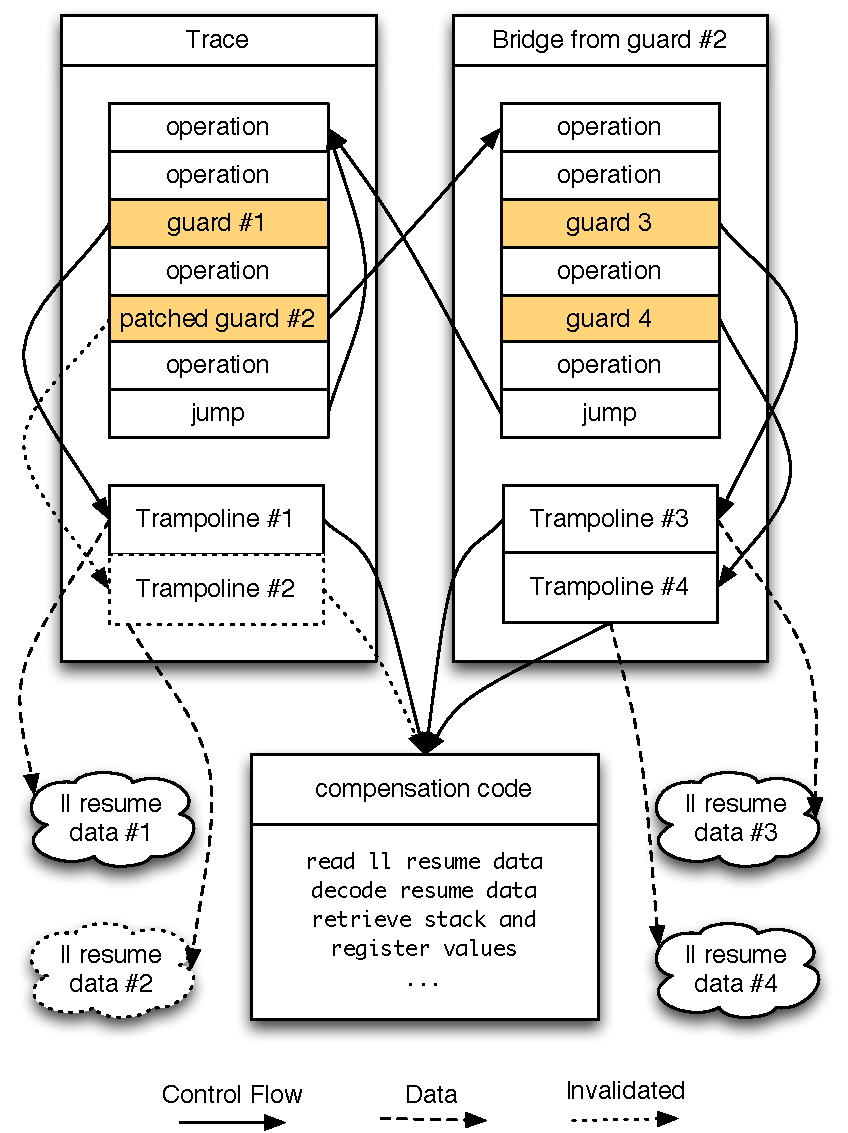
\includegraphics[width=0.5\textwidth]{figures/loop_bridge.pdf}
\caption{Trace control flow in case of guard failures with and without bridges}
\label{fig:trampoline}
\end{figure}
%* Low level handling of guards
%   * Fast guard checks v/s memory usage
%   * memory efficient encoding of low level resume data
%   * fast checks for guard conditions
%   * slow bail out
%
% section Guards in the Backend (end)

%___________________________________________________________________________


\section{Evaluation}
\label{sec:evaluation}

The results presented in this section are based on numbers gathered by running
a subset of the standard PyPy benchmarks. The PyPy benchmarks are used to
measure the performance of PyPy and are composed of a series of
micro-benchmarks and larger programs.\footnote{http://speed.pypy.org/} The
benchmarks were taken from the PyPy benchmarks repository using revision
\texttt{ff7b35837d0f}.\footnote{https://bitbucket.org/pypy/benchmarks/src/ff7b35837d0f}
The benchmarks were run on a version of PyPy based on the
tag~\texttt{0b77afaafdd0} and patched to collect additional data about the
guards in the machine code
backends.\footnote{https://bitbucket.org/pypy/pypy/src/0b77afaafdd0} All
benchmark data was collected on a MacBook Pro 64 bit running Max OS 10.8 with
the loop unrolling optimization disabled.\footnote{Since loop unrolling
duplicates the body of loops it would no longer be possible to meaningfully
compare the number of operations before and after optimization. Loop unrolling
is most effective for numeric kernels, so the benchmarks presented here are not
affected much by its absence.}

\todo{a description about what each selected benchmark does}

From the mentioned benchmarks we collected different datasets to evaluate the
Frequency, the overhead and overall behaviour of guards.
Figure~\ref{fig:benchmarks} summarizes the total number of operations that were
recorded during tracing for each of the benchmarks and what percentage of these
operations are guards. The number of operations was counted on the unoptimized
and optimized traces. Showing that the overall optimization rate is between
65.80\% and 86.23\% of all operations and that the optimization rate for guards
is similar to the general one, as could be assumed based on
Figure~\ref{fig:guard_percent}. These numbers show that guards are a rather
common operation in the traces, which is a reason the put effort into
optimizing them.
\todo{some pie charts about operation distribution}

\begin{figure*}
    \include{figures/benchmarks_table}
    \caption{Benchmark Results}
    \label{fig:benchmarks}
\end{figure*}

\todo{figure about failure counts of guards (histogram?)}
\todo{add resume data sizes without sharing}
\todo{add a footnote about why guards have a threshold of 100}

The overhead that is incurred by the JIT to manage the \texttt{resume data},
the \texttt{low-level resume data} as well as the generated machine code is
shown in Figure~\ref{fig:backend_data}. It shows the total memory consumption
of the code and of the data generated by the machine code backend and an
approximation of the size of the \texttt{resume data} structures for the
different benchmarks mentioned above. The size of the machine code is composed
of the size of the compiled operations, the trampolines generated for the
guards and a set of support functions that are generated when the JIT starts
and are shared by all compiled traces. The size of the \texttt{low-level resume
data} is the size of the compressed mapping from registers and stack to
IR-level variable and finally the size of the \texttt{resume data} is an
approximation of the size of the compressed high-level resume data\todo{explain
why it is an approximation}.

Compared to the size of the generated machine code the compressed
\texttt{low-level resume data} is about 15\% to 20\% of that size, depending on
the benchmark. On the other hand the generated machine code has only a size
ranging from 20.21\% to 37.98\% of the size of the high and low-level
\texttt{resume data} being compressed as described before.

Tracing JIT compilers only compile the subset of the code executed in a program
that is traced in a hot loop, for this reason the amount of generated machine
code will be smaller than in other juts-in-time compilation approaches. Still
the overhead associated to guards to resume execution from a side exit appears
to be high.\bivab{put into relation to other JITs, compilers in general}

\begin{figure*}
    \include{figures/backend_table}
    \caption{Total size of generated machine code and guard data}
    \label{fig:backend_data}
\end{figure*}

Both figures do not take into account garbage collection. Pieces of machine
code can be globally invalidated or just become cold again. In both cases the
generated machine code and the related data is garbage collected. The figures
show the total amount of operations that are evaluated by the JIT and the
total amount of code and data that is generated from the optimized traces.

\todo{compare to naive variant of resume data}
\todo{Measure the of guards and how many of these ever fail}

\section{Related Work}
\label{sec:Related Work}

\subsection{Guards in Other Tracing JITs}
\label{sub:Guards in Other Tracing JITs}

Guards as described are a concept associated with tracing just-in-time
compilers to represent possible divergent control flow paths.

SPUR~\cite{bebenita_spur:_2010} is a tracing JIT compiler
for a C\# virtual machine.
It handles guards by always generating code for every one of them
that transfers control back to the unoptimized code.
Since the transfer code needs to reconstruct the stack frames
of the unoptimized code,
the transfer code is quite large.

Mike Pall, the author of LuaJIT describes in a post to the lua-users mailing
list different technologies and techniques used in the implementation of
LuaJIT~\cite{Pall:2009}.\todo{decide if LuaJIT is a footnote or a reference and
fix website citation} Pall explains that guards in LuaJIT use a datastucture
called snapshots, similar to PyPy's resume data, to store the information about
how to rebuild the state from a side-exit using the information in the snapshot
and the machine execution state. Pall also acknowledges that snapshot for
guards are associated with a large memory footprint. The solution used in
LuaJIT is to store sparse snapshots, avoiding the creation of snapshots for
every guard to reduce memory pressure. Snapshots are only created for guards
after updates to the global state, after control flow points from the original
program and for guards that are likely to fail. As an outlook Pall mentions the
plans to switch to compressed snapshots to further reduce redundancy.

Linking side exits to pieces of later compiled machine code was described first
in the context of Dynamo~\cite{Bala:2000wv} under the name of Fragment Linking.
Once a new hot trace is emitted into the fragment cache it is linked to side
exit that led to the compilation. Fragment Linking avoids the performance
penalty involved in leaving the compiled and it to remove the compensation
code used when restoring the machine state on a side exit.

In~\cite{Gal:2006} Gal et. al describe that in the HotpathVM they experimented
with having one generic compensation code block, like the RPython JIT, that
uses a register variable mapping to restore the interpreter state. Later this
was replaced by generating compensation code for each guard which produced a
lower overhead in their benchmarks. HotpathVM also records secondary traces
starting from failing guards that are connected directly to the original trace.
Secondary traces are compiled by first restoring the register allocator state to
the state at the side exit. The information is retrieved from a mapping stored
in the guard that maps machine level registers and stack to Java level stack
and variables.

Gal et. al~\cite{Gal:2009ux} write about how TraceMonkey uses trace stitching
to avoid th overhead of returning to the trace monitor and calling another
trace when taking a side exit. In their approach it is required to write live
values to an activation record before entering the new trace.

% subsection Guards in Other Tracing JITs (end)

\subsection{Deoptimization in Method-Based JITs}
\label{sub:Deoptimization in Method-Based JITs}

Deoptimization in method-based JITs is used if one of the assumptions
of the code generated by a JIT-compiler changes.
This is often the case when new code is added to the system,
or when the programmer tries to debug the program.

Deutsch et. al.~\cite{deutsch_efficient_1984} describe the use of stack descriptions
to make it possible to do source-level debugging of JIT-compiled code.
Self uses deoptimization to reach the same goal~\cite{XXX}.
When a function is to be debugged, the optimized code version is left
and one compiled without inlining and other optimizations is entered.
Self uses scope descriptors to describe the frames
that need to be re-created when leaving the optimized code.
The scope descriptors are between 0.45 and 0.76 times
the size of the generated machine code.

Java Hotspot~\cite{paleczny_java_2001} contains a deoptimization framework that is used
for debugging and when an uncommon trap is triggered.
To be able to do this, Hotspot stores a mapping from optimized states
back to the interpreter state at various deoptimization points.
There is no discussion of the memory use of this information.

The deoptimization information of Hotspot is extended
to support correct behaviour
when scalar replacement of fields is done for non-escaping objects~\cite{kotzmann_escape_2005}.
The approach is extremely similar to how RPython's JIT handles virtual objects.
For every object that is not allocated in the code,
the deoptimization information contains a description
of the content of the fields.
When deoptimizing code, these objects are reallocated
and their fields filled with the values
described by the deoptimization information.
The paper does not describe any attempts to store this information compactly.


% subsection Deoptimization in Method-Based JITs (end)
% section Related Work (end)


\section{Conclusion}
\label{sec:Conclusion}

\todo{conclusion}

\section*{Acknowledgements}
\section*{Appendix}
\begin{figure*}
    \include{figures/ops_count_table}
    \caption{Relative numbers of operations in the traces generated for
    different benchmarks}
    \label{fig:ops_count}
\end{figure*}
\begin{figure*}
\centering
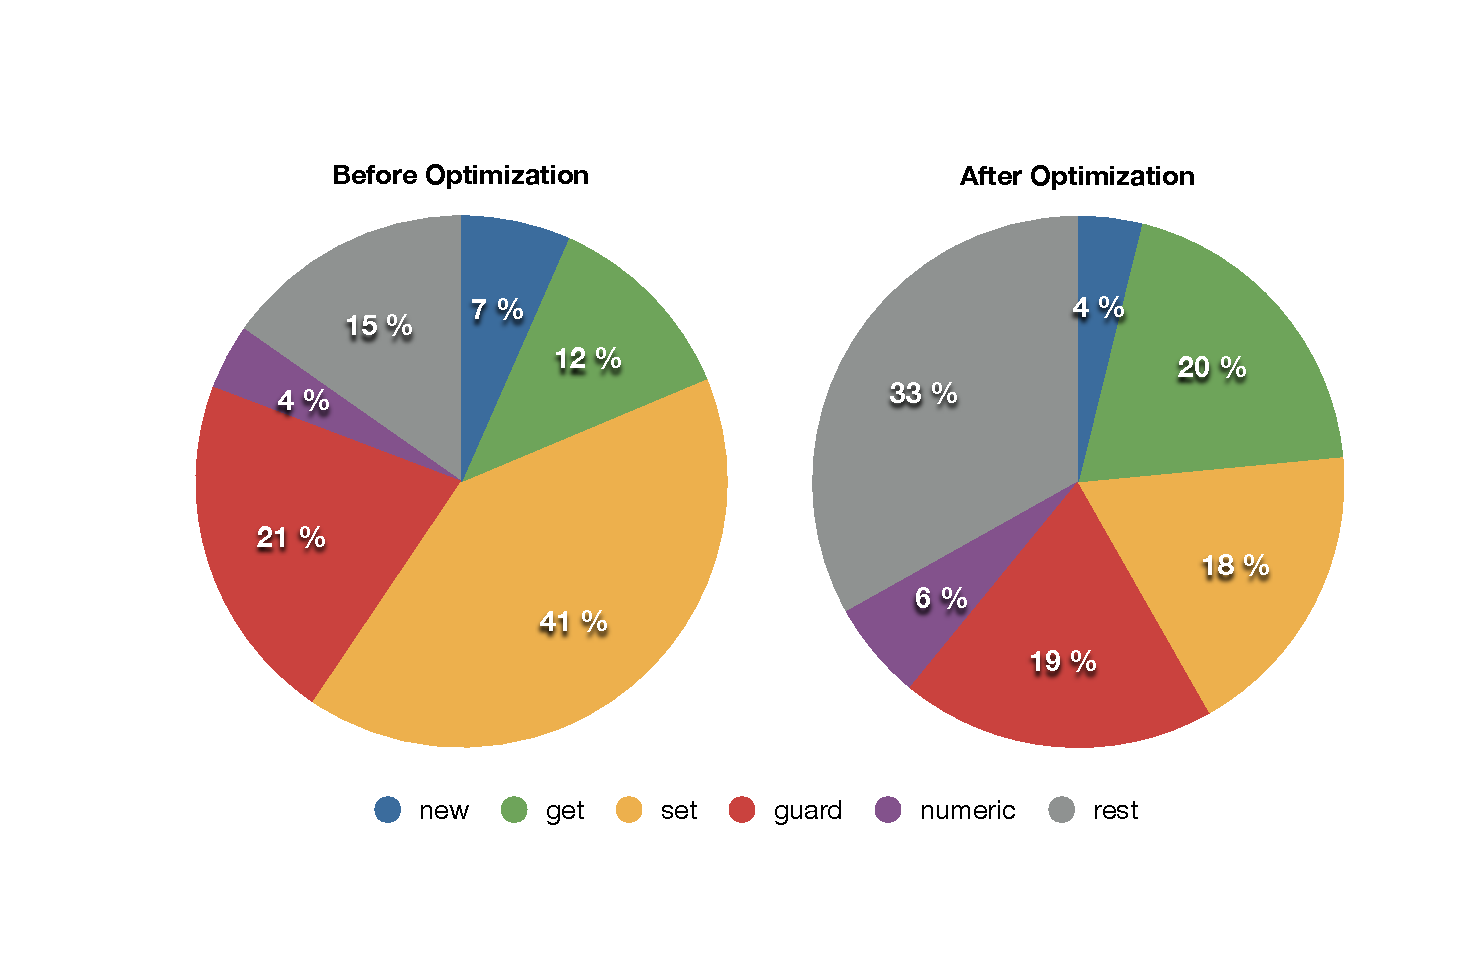
\includegraphics[width=\textwidth]{figures/ops_pie.pdf}
\caption{Relative frequency of operations before and after optimization}
\label{fig:ops_pie}
\end{figure*}
\bibliographystyle{abbrv}
\bibliography{zotero,paper}
\listoftodos
\end{document}
